\documentclass[tikz,border=8pt]{standalone}

\usepackage[T1]{fontenc}
\usepackage{lmodern}
\usetikzlibrary{arrows.meta,calc,positioning}

\definecolor{neutralfill}{RGB}{246,245,241}
\definecolor{modelfill}{RGB}{241,240,255}
\definecolor{analysisfill}{RGB}{236,249,246}

\begin{document}
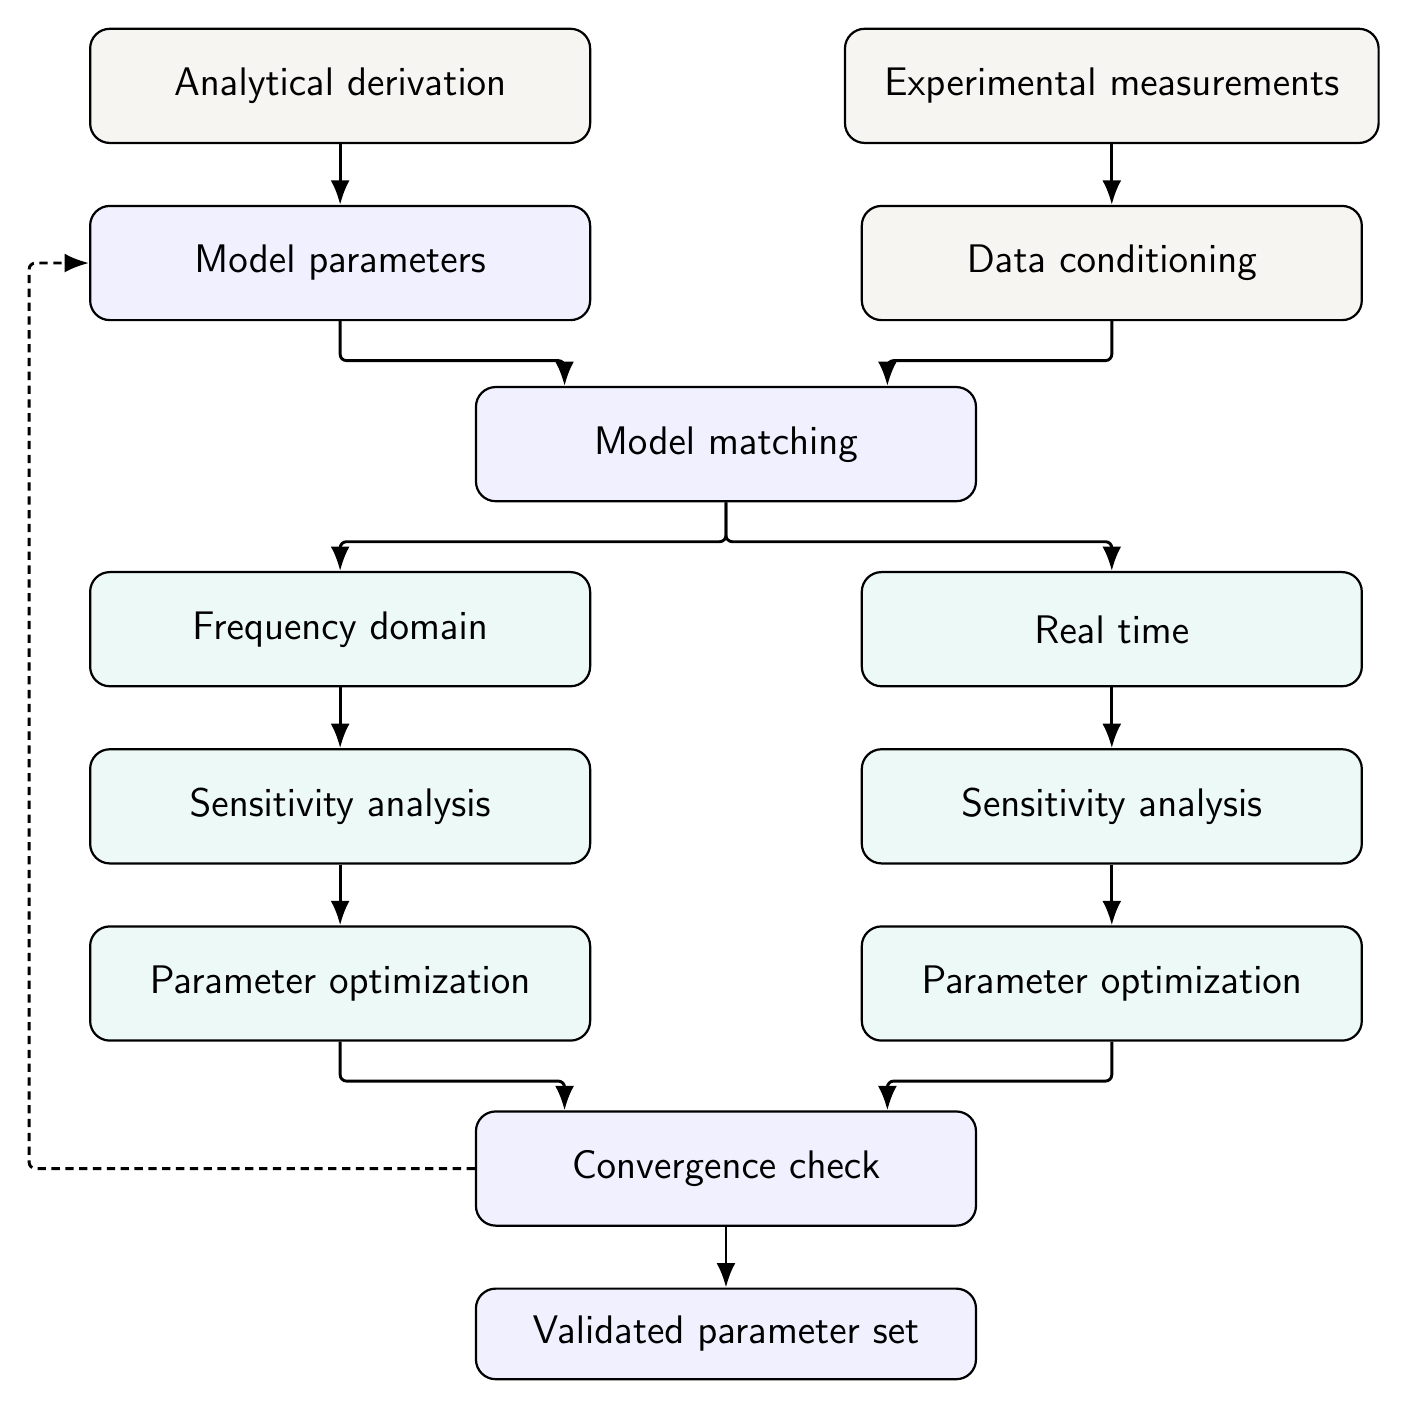
\begin{tikzpicture}[
  font=\sffamily,
  block/.style={
    draw=black,
    line width=0.8pt,
    rounded corners=2.5mm,
    minimum width=6.35cm,
    minimum height=1.45cm,
    inner xsep=5mm,
    inner ysep=3mm,
    align=center,
    text=black
  },
  neutral/.style={block,fill=neutralfill},
  model/.style={block,fill=modelfill},
  analysis/.style={block,fill=analysisfill},
  flow/.style={
    draw=black,
    line width=1.05pt,
    -{Latex[length=3.1mm,width=2.4mm]},
    rounded corners=0.8mm
  },
  feedback/.style={
    flow,
    densely dashed
  }
]

% Inputs and preparation
\node[neutral] (derivation) at (-4.9,0)
  {\Large Analytical derivation};
\node[neutral] (measurements) at (4.9,0)
  {\Large Experimental measurements};

\node[model] (parameters) at (-4.9,-2.25)
  {\Large Model parameters};
\node[neutral] (conditioning) at (4.9,-2.25)
  {\Large Data conditioning};

\node[model] (matching) at (0,-4.55)
  {\Large Model matching};

% Parallel residual definitions
\node[analysis] (frequency) at (-4.9,-6.90)
  {\Large Frequency domain};
\node[analysis] (realtime) at (4.9,-6.90)
  {\Large Real time};

\node[analysis] (sensitivity-f) at (-4.9,-9.15)
  {\Large Sensitivity analysis};
\node[analysis] (sensitivity-t) at (4.9,-9.15)
  {\Large Sensitivity analysis};

\node[analysis] (optimisation-f) at (-4.9,-11.40)
  {\Large Parameter optimization};
\node[analysis] (optimisation-t) at (4.9,-11.40)
  {\Large Parameter optimization};

% Convergence and output
\node[model] (convergence) at (0,-13.75)
  {\Large Convergence check};
\node[model,minimum height=1.15cm] (validated) at (0,-15.85)
  {\Large Validated parameter set};

% Flow connectors
\draw[flow] (derivation.south) -- (parameters.north);
\draw[flow] (measurements.south) -- (conditioning.north);

\draw[flow] (parameters.south) -- ++(0,-0.50) -|
  ([xshift=-2.05cm]matching.north);
\draw[flow] (conditioning.south) -- ++(0,-0.50) -|
  ([xshift=2.05cm]matching.north);

\draw[flow] (matching.south) -- ++(0,-0.50) -| (frequency.north);
\draw[flow] (matching.south) -- ++(0,-0.50) -| (realtime.north);

\draw[flow] (frequency.south) -- (sensitivity-f.north);
\draw[flow] (realtime.south) -- (sensitivity-t.north);
\draw[flow] (sensitivity-f.south) -- (optimisation-f.north);
\draw[flow] (sensitivity-t.south) -- (optimisation-t.north);

\draw[flow] (optimisation-f.south) -- ++(0,-0.50) -|
  ([xshift=-2.05cm]convergence.north);
\draw[flow] (optimisation-t.south) -- ++(0,-0.50) -|
  ([xshift=2.05cm]convergence.north);
\draw[flow] (convergence.south) -- (validated.north);

% Failed convergence returns to the parameter definition.
\draw[feedback] (convergence.west) -- (-8.85,-13.75) |-
  (parameters.west);

\end{tikzpicture}
\end{document}
